\documentclass[letterpaper,twocolumn,10pt]{article}
\usepackage{usenix2019_v3}
\usepackage{tikz}
\usepackage{minted}
\usepackage{amsmath}

\newcommand{\citeme}{}

%-------------------------------------------------------------------------------
\begin{document}
%-------------------------------------------------------------------------------

\title{\Large \bf An Easy and Safe Implementation of Truly Parallel Threads in CPython}

\author{
{\rm Samuel Grayson}\\
University of Illinois at Urbana-Champaign
}

\maketitle

%-------------------------------------------------------------------------------
\begin{abstract}
% -------------------------------------------------------------------------------

  Mutually trusting processes can be safely run in the same address-space (effectively running \textbf{processes-as-threads}) without necessitating source-code changes.
  This has compelling performance improvements for programs that can be realized with very little work.
  Some programs such as Python do not support parallel threads, and this may be the only easy way to unlock high performance on multicore architecture.

  In just one semester I have implemented a prototype of the process-as-threads abstraction for CPython, which allows it to run parallel threads safely.
  The performance characteristics are promising, and it seems to scale better than the state-of-the-art with a large number of cores.
\end{abstract}

%-------------------------------------------------------------------------------
\section{Motivation}
%-------------------------------------------------------------------------------

While distinct virtual-to-physical mappings (\textbf{address space}) for several reasons are extremely important in the general case, 
I argue that there is a specific case where we can relax them for the sake of performance.
Multithreading and virtual memory-aliasing (\texttt{mmap}) already relax this constraint in \textit{non}-memory-safe languages, which is more dangerous than my proposal.

\begin{description}
\item[Stability]
  One malfunctioning process should not be able to cause other processes to malfunction\citeme.
  When a programmer wants to parallelize code, they implicitly trust themselves, so the security of processes is not necessary here\citeme.
\item[Security]
  Processes do not necessarily trust each other with their volatile data\citeme.
  In a memory-safe programming languages, direct memory access is not possible, eliminating this class of bugs\citeme.
\end{description}

On the other hand, running in the same address space has important performance benefits:

\begin{description}
\item[Reduced context-switching time]
  When the OS switches from one process to another it has to flush the TLB, file-descriptor table, and other per-process resources;
  When switching between threads, this state is shared\citeme.
\item[Reduced communication/synchronization time]
  Inter-process communication (such as a Unix pipe) has to copy data into and out-from the kernel;
  Inter-thread communication can leverage the shared memory-space, copying the data once or zero times (sending a reference)\citeme.
\item[Reduced memory fragmentation]
  Huge pages are intended to extend the reach of the TLB, however this faces implementation problems.
  If each process gets a huge page, physical memory runs out, even though each process might only be using a fraction of its page.
  Multiple threads however could share a huge page between themselves\citeme.
\end{description}

Parallel workloads are becoming increasingly important due to the limitations of single-core performance and the move to multi-core\citeme.
While challenging, this is much more practical for many users than setting up a distributed system.
That is why I am interested in making multi-core programming easier to do with existing paradigms.

Python is an obvious place to start.
The Jupyter Notebook interface explicitly targets data-scientists and tools like Numpy, Scipy, and Pandas are extremely popular tools for data analytics.
However Python fails to harness multicore parallelism with shared memory.
If it could do this, then it would accelerate a lot of real-world workloads from big companies.
Every Spark-node could be utilizing process-as-threads to accelerate intra-node data-transfers on many-core machines like the Xeon Phi.
% While Python is not built to address performance like a compiled-language, beca

Python cannot support parallel multithreading because it is not threadsafe\citeme.
There is a \textbf{Global Interpreter Lock (GIL)} ensuring only one thread of Python bytecode is executing at a time\citeme.
It has a \texttt{threading}~\citeme module, but it is limited by the GIL.
The state-of-the-art for Python is to use the \texttt{multiprocessing}~\citeme module\citeme.
While this achieves true parallelism, it leaves a lot of performance on the table (slow context-switching, slow communcation, and poor memory fragmentation) because the process abstraction is so heavy-weight.

Many other interpreted-languages, such as Ruby, have a GIL as well.
In these lanuages, neither normal processes nor normal threads can provide the benefits of running in the same address-space.

%-------------------------------------------------------------------------------
\section{Process-as-Threads Programming Model}
%-------------------------------------------------------------------------------

My vision is to spawn multiple processes in the same address-space such that they do not interfere with each other.
This has important implications for each memory segment: text, static, initialized, heap, and stack.

\begin{description}
\item[text]
Function-calls are implemented by jumping to the virtual-address containing the function.
As a consequence, when the compiler lays out the binary, it tells the loader to load each piece of executable code into a specific virtual-address.
It will hardcode that address later at every function-call site.
Imagine A wants to install \texttt{foo()} at 0xDEADBEEF and B wants to install \texttt{bar()} at the same address.

My solution is to use \textbf{Position-Independent Code (PIC)} and shared-libraries\citeme.
When PIC is enabled, compilers add an extra layer of indirection: they first go to a table which is located by its address \textit{relative} to the \$PC. This \textbf{Global-offset Table (GOT)} contains the real address of the desired function.
When linking as a shared-library, the code can be loaded anywhere, as long as the loader also updates the GOT.

\item[static]
The same problem occurs for static and initialized global variables.
The compiler normally hard-codes virtual-addresses to static variables.
However, the same solution also works:
The shared-library loader updates a GOT accessible by relative address.
% Unfortunately this causes an unnecessary increase in the memory-usage of the entire process when copies of the same program are being run.
% However, the same function would need to refer to a different set of static variables for different threads, so working off of one copy of the code for all threads is difficult.
% I am considering designs that have the code shared (not-copied) but have the global lookup-table in thread-local storage.

\item[heap]
I need to show that the programs don't interfere with each-other's heap space.
I can prove this by observing that a memory-safe program never accesses (read or write) memory that never allocated first.
As long as the memory-allocator is aware of multiple threads and does not return the same memory for multiple threads, then the programs will always allocate objects in non-conflicting places on the heap.
The heap is logically partitioned (each object is only referenced by one thread) despite it not being literally partitioned in virtual-address space.

When I require that memory-safe accesses, I am not requiring any property of the \textit{user's code}, just the \textit{interpreter's code}.
At this point, the Python interpreter is considered mature and usually user-code crashes, not its code.

\item[stack]
With the other segments out of the way, it is safe to use threads.
Threads give us independent stack-segments.
\end{description}

Despite having the \textit{performance benefit of threads}, the process-as-thread programming model has the \textit{strong semantics of processes}.
With multithreading, each thread has to reason about another thread modifying all of its data, because other threads can take references to any thread's data.
With processes-as-threads, data is not referencible from other process-as-threads by default.
This is surprising considering that they run in the same address space, but if the code is written in a memory-safe language, it is impossible to take a reference to data from another process-as-thread without explicit permission.
Where it is expedient, processes-as-threads can \textit{explicitly} send a reference to another process-as-thread.
This is a useful for the underlying runtime to do when it is safe (e.g. providing read-only access to a global constant).
Because privacy is not default, it does not burden the programmer with complex memory semantics, race conditions, and deadlocks.

%-------------------------------------------------------------------------------
\section{Python Implementation}
%-------------------------------------------------------------------------------

In Python, a CPU-bound parallel work is often done using the \texttt{multiprocessing} library.
It provides low-level primitives such actors, queues, and pipes, but also high-level abstractions such as a process pool.
I could attempt to make process-as-threads emulate the low-level primitives, but instead I just attempted to provide the high-level abstractions with process-as-threads.
Because my interface is the same, users only have to change one line of code to reference my library instead of the default \texttt{multiprocessing} library.
Furthermore, accelerating a higher-order primitive means that I can transparently easily replace the interprocess-communication going on the background with fast interthread-communication.

Now I have the problem of non-atomic reference-counting.
Two concurrent threads trying to change the reference-count of the same variable is a race-condition, which could render the whole program incorrect.
To avoid this I deepcopy every object immediately before it gets sent to another thread.
That way both threads have a copy of the object, but each thread only references its copy.
Deepcopying is somewhat expensive, but is strictly cheaper than to serialization/deserialization, which is what multiprocessing usually has to do to communicate.
Processes-as-thread's communication is cheaper in other ways: thye do not have to invoke a syscall to send a message.
Note that immutable data-types such as strings, tuples, functions, and primitives \textit{are not even copied at all}: when \texttt{deepcopy} encounters these, it just returns the original pointer. Since the destination is in the same address-space, this works without modification!

Now, my safety is guaranteed by the invariant that every object has references in at most one thread.
The following three operations maintain the invariant:
\begin{itemize}
\item Allocating
\item Deallocating
\item Taking a reference within the same thread
\item Copying within the same thread
\item Deepcopy+send between threads
\end{itemize}

See Appendix \ref{appendix:availability} for implementation details.

%-------------------------------------------------------------------------------
\section{Empirical Results}
%-------------------------------------------------------------------------------

I tested this on a program that counts up to a large number, call it \(n\).
When this is parallelized, each of \(m\) actors has to count to \(\lfloor \frac{n}{m} \rfloor\)
The only communication is starting up the actors, telling them the number, and then waiting for them to finish.
I ran it with process-parallelization (\texttt{proc}), a thread-parallelization (\texttt{thread}), and a process-as-thread parallelization (\texttt{pat}).

Figure \ref{fig:count_runtime} shows how the performance scales to many cores.
Thread-parallelization actual gets worse when we add more cores.
This demonstrates the GIL's limitation on Python's existing threading facilities.
Process-as-threads and processes both scale well with these conditions, demonstrating truly parallel (not just concurrent) execution.

\begin{figure}
\begin{center}
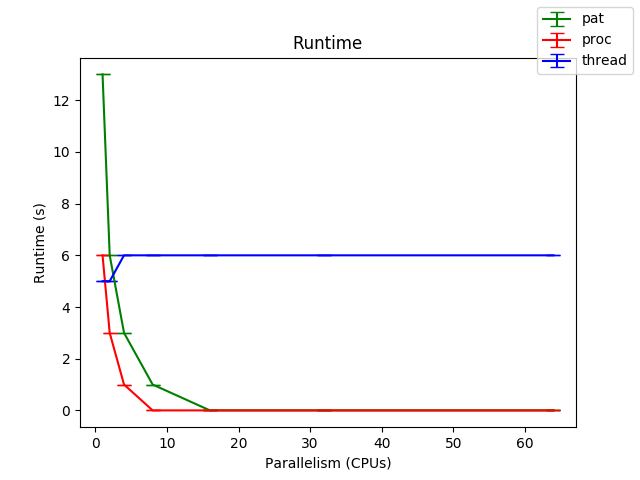
\includegraphics[width=\textwidth / 2]{total_runtime.png}
\end{center}
\caption{\label{fig:count_runtime} }
\end{figure}

However, the lines get close together, so it is hard to tell how the performance scales at 64 cores.
This is more apparent in the speedup-over-baseline in Figure \ref{fig:count_speedup}.
We see that process-as-threads totally outperforms processes with a very high number of CPU.
The error-bars are very high because the runtimes are close to zero, so small absolute deviations blow up after taking the reciprocal.

\begin{figure}
\begin{center}
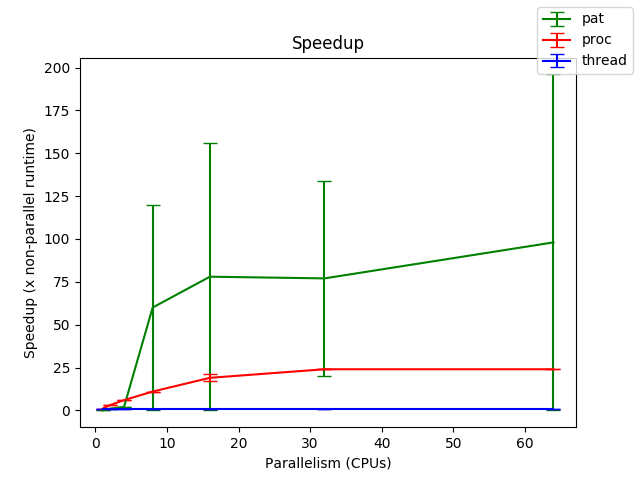
\includegraphics[width=\textwidth / 2]{total_speedup.png}
\end{center}
\caption{\label{fig:count_speedup} }
\end{figure}

This test does stress communication at all, which should only be more compelling for process-as-threads.

See Appendix \ref{appendix:conditions} for my experimental conditions and Appendix \ref{appendix:availability} to reproduce.

%-------------------------------------------------------------------------------
\section{Unresolved Issues}
%-------------------------------------------------------------------------------

There is an unresolved issue that prevents Python imports from working properly.
Usually when one loads shared-library, call it libA, libA's symbols are exported globally.
This means that when a subsequent shared-library are loaded, call it LibB, their undefined symbols are resolved within libA.
When an application loads Python, calls it to run a script, and that script loads a C-extension, the C-extension expects its undefined symbols to be resolved within Python.

However, this poses a problem for process-as-threads.
Remember that each process-as-thread loaded its own copy of Python, so it could get its own copy of the text and static variables.
Now when libB gets loaded, which library should its undefined symbols be resolved in?
There is no POSIX compliant way of opening a shared-library and capturing its names in a namespace.
One either has to export them globally or not at all through \texttt{dlopen}.

However Linux does offer such a facility: \texttt{dlmopen}.
You can open a library \textit{inside} a non-default namespace; its symbols get added to this namespace, and its undefined symbols are resolved in that namespace.
Then I could make each thread have its own namespace object, and I would ensure that all libraries that would be loaded globally get loaded into that namespace object instead.
Now when libB needs to be loaded, its unresolved symbols can be found in the calling thread's namespace object.
But for some reason this is not working, and it is causing Python to crash when it attempts to import a C-module.

%-------------------------------------------------------------------------------
\section{Conclusion}
%-------------------------------------------------------------------------------


  In just one semester I have implemented a prototype of the process-as-threads abstraction.
  I have been able to show promising performance benefits on a software project as mature as Python, in little time and with little experience.
  The process-as-threads abstraction can provide this benefit without modifying CPython nor the OS kernel at all.
  Compare this to other proposals which involve a massive overhaul of the CPython interpreter--a so-called `GIL-ectomy'.

  My vision is that with one more year I could develop a polished process-as-threads which could parallelize any programming language interpreter without any change to process-as-threads or the language.
  My work could even apply to run two different lanuage interpreters in the same addres-space, accelerating polyglot applications (i.e. a system utilizing code in multiple languages simultaneously).

%-------------------------------------------------------------------------------
\section*{Appendex}
%-------------------------------------------------------------------------------

%-------------------------------------------------------------------------------
\subsection{Availability}\label{appendix:availability}
%-------------------------------------------------------------------------------

To reproduce:

\begin{enumerate}
\item Clone the code from here \url{https://github.com/charmoniumQ/exec_sharing/}
\item Switch to branch \texttt{dlib-load-no-libs}.
\item Run \texttt{./bootstrap\_debian.sh} to prepare your machine. It should be running a recent Debian.
  \begin{enumerate}
  \item Be aware that the script will irrevocably uprade to Debian Testing. This is because my code needs a recent version of clang.
  \end{enumerate}
\item Run \texttt{./perf/count.sh} to reproduce the performance tests.
  \begin{enumerate}
  \item Run \texttt{./perf/plots.py} to produce the plots.
  \item If you would like to try your own performance test with process-as-threads, mimic \texttt{./perf/count\_pat.py}.
  \end{enumerate}
\item Run \texttt{make tests} to run functional tests.
  \begin{enumerate}
  \item If you would like to write your own functional tests, mimic those in \texttt{./tests/test\_*.sh}.
  \end{enumerate}
\end{enumerate}

% %-------------------------------------------------------------------------------
% \subsection{Implementation Details}\label{appendix:implementation}
% %-------------------------------------------------------------------------------

% \begin{enumerate}
% \item \texttt{p = multiprocessing.Pool()} is called. I will call this thread the ``main thread''.
% \item \texttt{multiprocessing.Pool} starts several Queues.
% \item \texttt{multiprocessing.Pool} spawns new threads, sending the address of the queue as a command-line argument.
% \item Each thread runs a copy of the Python interpreter.
% \item Each thread loads a queue from the address they got on the command-line.
% \item \texttt{p.map(func, iterable)} is called.
% \item This thread deepcopies chunks of the \texttt{iterable} and pushes it onto queues for the worker threads to pull from.
% \item Worker threads deepcopy their result and push it on a queue for the main thread to pull from.
% \item \texttt{p.map(func, iterable)} returns that result.
% \end{enumerate}

% Communicating between threads is non-trivial because even though the processes-as-threads start in the same address-space, they don't have any shared variables.
% I start process-as-threads by invoking Python's main method, which accepts command-line arguments.
% I got around this by creating a queue, writing its address as a command-line argument to the other threads, starting up the other threads, reading the address from command-line, and finding the queue there.

%-------------------------------------------------------------------------------
\subsection{Experimental Conditions}\label{appendix:conditions}
%-------------------------------------------------------------------------------

I used an AWS c5.18xlarge (72-core) with Intel(R) Xeon(R) Platinum 8124M CPU @ 3.00GHz.

A smaller machine would probably be more appropriate, because I did not max out the cores.

I used \texttt{taskset} to ensure the processes did not migrate threads.

I used \texttt{perf} to capture total-time. I decided not to present user-time and system-time separately because they were unstable.

% %-------------------------------------------------------------------------------
% \subsection{Lower-level Usage}
% %-------------------------------------------------------------------------------

% The programmer writes code as usual for multiple cooperating processes.

% \definecolor{bg}{rgb}{0.95,0.95,0.95}
% \begin{minted}[bgcolor=bg]{c}
% // proc1.c
% int main() {
%   // talk to proc2
% }
% \end{minted}

% \begin{minted}[label=proc2,bgcolor=bg]{c}
% // proc2.c
% int main() {
%   // talk to proc1
% }
% \end{minted}

% Suppose she normally runs them as backround processes

% \begin{minted}[bgcolor=bg]{shell}
% $ ./proc1 &
% $ ./proc2 &
% \end{minted}

% She needs only recompile with shared-library and PIC flags, and she can run them together, without changing the code at all.
% I could also use LD_PRELOAD to transparently turn slow inter-process communication into fast inter-thread communication.

% \begin{minted}[bgcolor=bg]{shell}
% $ ./exec_sharing ./proc1 \; ./proc2
% $ # proc1 and proc2 execute as threads
% $ # in the same address space.
% \end{minted}
% % $

% %-------------------------------------------------------------------------------
% \subsection{Failed Attempts}
% %-------------------------------------------------------------------------------

% \bibliographystyle{plain}
% \bibliography{\jobname}

\end{document}
%%% Local Variables:
%%% mode: latex
%%% TeX-master: t
%%% End:
